% DMA Session 5: Warum mehrere Tabellen?
% 180-Minuten-Block (Vorlesung + Übung interwoven)

\documentclass[usenames,dvipsnames,10pt,aspectratio=169]{beamer}
\usepackage[T1]{fontenc}
\usepackage[utf8]{inputenc}
\usepackage{verbatim}

% Theme loaded via symlinks (update beamerTemplate/ for CD changes)
\usetheme{ims}

\usepackage{booktabs}
\usepackage{multicol}
\usepackage{listings}
\usepackage{xcolor}
\usepackage{graphicx}
\usepackage{tikz}
\usepackage{colortbl}
\usetikzlibrary{shapes.geometric, arrows.meta, positioning, calc, fit, backgrounds, matrix, shapes.multipart}

% TikZ styles for diagrams
\tikzset{
    sqlbox/.style={rectangle, rounded corners, minimum width=2.5cm, minimum height=0.8cm,
        text centered, draw=IMSBlue, fill=IMSBlue!15, font=\ttfamily\small},
    sqlarrow/.style={-{Stealth[length=2.5mm]}, thick, IMSOrange},
    databox/.style={rectangle, minimum width=1.2cm, minimum height=0.5cm,
        text centered, draw=gray, fill=gray!10, font=\small},
    alertbox/.style={rectangle, rounded corners, minimum width=2cm, minimum height=0.6cm,
        text centered, draw=red!70, fill=red!15, font=\small},
    goodbox/.style={rectangle, rounded corners, minimum width=2cm, minimum height=0.6cm,
        text centered, draw=green!60!black, fill=green!15, font=\small},
    entitybox/.style={rectangle, minimum width=2.5cm, minimum height=1cm,
        text centered, draw=IMSBlue, fill=IMSBlue!15, font=\bfseries},
    relationbox/.style={diamond, aspect=2, minimum width=1.5cm,
        text centered, draw=IMSOrange, fill=IMSOrange!15, font=\small},
    tablecell/.style={rectangle, minimum width=2cm, minimum height=0.5cm,
        draw=gray, font=\small},
    redundant/.style={fill=red!20},
    normal/.style={fill=green!10},
    badtable/.style={draw=red!70, thick},
    goodtable/.style={draw=green!60!black, thick},
}

% SQL Listing Style
\lstdefinestyle{sql}{
    language=SQL,
    basicstyle=\ttfamily\footnotesize,
    keywordstyle=\color{IMSBlue}\bfseries,
    stringstyle=\color{IMSOrange},
    commentstyle=\color{gray}\itshape,
    showstringspaces=false,
    breaklines=true,
    frame=single,
    backgroundcolor=\color{gray!10},
    morekeywords={SERIAL, BOOLEAN, TEXT, COALESCE, SUBSTR, CAST, LOG10, FLOOR, ABS},
    literate={ü}{{\"u}}1 {ä}{{\"a}}1 {ö}{{\"o}}1 {Ü}{{\"U}}1 {Ä}{{\"A}}1 {Ö}{{\"O}}1 {ß}{{\ss}}1
}

\lstset{style=sql}

% ===== CLICKABLE AGENDA WITH PROGRESS INDICATOR =====
\usepackage{hyperref}
\hypersetup{colorlinks=false, pdfborder={0 0 0}}

% Phase counter for progress tracking
\newcounter{currentphase}
\setcounter{currentphase}{0}

% Clickable agenda item
\newcommand{\agendaitem}[3]{%
    \ifnum#1=#2
        \textcolor{IMSOrange}{$\blacktriangleright$ \textbf{\hyperlink{phase#2}{#3}}}%
    \else
        \textcolor{gray!70}{\phantom{$\blacktriangleright$} \hyperlink{phase#2}{#3}}%
    \fi\\[0.3em]%
}

% Progress dots for footline (clickable)
\newcommand{\progressdots}{%
    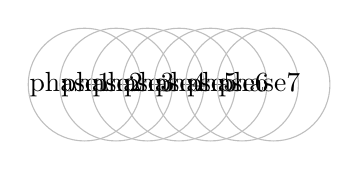
\begin{tikzpicture}[baseline=-0.5ex]
        \foreach \i in {1,...,7} {
            \ifnum\value{currentphase}=\i
                \node[circle, fill=IMSOrange, minimum size=0.24cm, inner sep=0pt] at (\i*0.4,0) {\hyperlink{phase\i}{\phantom{oo}}};
            \else
                \ifnum\value{currentphase}>\i
                    \node[circle, fill=IMSBlue!60, minimum size=0.2cm, inner sep=0pt] at (\i*0.4,0) {\hyperlink{phase\i}{\phantom{oo}}};
                \else
                    \node[circle, draw=gray!50, minimum size=0.2cm, inner sep=0pt] at (\i*0.4,0) {\hyperlink{phase\i}{\phantom{oo}}};
                \fi
            \fi
        }
    \end{tikzpicture}%
}

% Add progress indicator to footline
\setbeamertemplate{footline}{%
    \leavevmode%
    \hbox{%
        \begin{beamercolorbox}[wd=.33\paperwidth,ht=2.5ex,dp=1ex,left]{author in head/foot}%
            \usebeamerfont{author in head/foot}\hspace*{2ex}\insertshortauthor
        \end{beamercolorbox}%
        \begin{beamercolorbox}[wd=.34\paperwidth,ht=2.5ex,dp=1ex,center]{title in head/foot}%
            \progressdots
        \end{beamercolorbox}%
        \begin{beamercolorbox}[wd=.33\paperwidth,ht=2.5ex,dp=1ex,right]{date in head/foot}%
            \usebeamerfont{date in head/foot}\insertframenumber{} / \inserttotalframenumber\hspace*{2ex}
        \end{beamercolorbox}%
    }%
    \vskip0pt%
}

% Agenda reminder frame - argument is the current phase number
\newcommand{\showagenda}[1]{%
\setcounter{currentphase}{#1}%
\hypertarget{phase#1}{}%
\begin{frame}{Agenda}
\vfill
\begin{center}
\begin{minipage}{0.7\textwidth}
\large
\agendaitem{#1}{1}{1 ~ Rückblick \& Motivation}
\agendaitem{#1}{2}{2 ~ Die ``Mega-Tabelle'' -- Ein Beispiel}
\agendaitem{#1}{3}{3 ~ Anomalien: Was schief gehen kann}
\agendaitem{#1}{4}{4 ~ Anomalien selbst erleben}
\agendaitem{#1}{5}{5 ~ Die Lösung: Daten aufteilen}
\agendaitem{#1}{6}{6 ~ Erste Schritte zur Modellierung}
\agendaitem{#1}{7}{7 ~ Zusammenfassung \& Ausblick}
\end{minipage}
\end{center}
\vfill
\end{frame}
}

%%%%%%%%%%%%%%%%%%%%%%%%%%%%%%%%%%%%%%%%%%%%%%%%%%%%%%%%%%%%%%%%%%%%%%%%%%%%%%%%%%%%%
\title[DMA 05]{Datenmanagement \& -analyse}
\subtitle{Vorlesung 5: Warum mehrere Tabellen?}
\date{Sommersemester 2026}
\author{Prof. Dr. Christoph M. Flath}
\institute{Data Driven Decisions Group, Universität Würzburg}
%%%%%%%%%%%%%%%%%%%%%%%%%%%%%%%%%%%%%%%%%%%%%%%%%%%%%%%%%%%%%%%%%%%%%%%%%%%%%%%%%%%%%

\begin{document}

\begin{frame}
\titlepage
\end{frame}

%%%%%%%%%%%%%%%%%%%%%%%%%%%%%%%%%%%%%%%%%%%%%%%%%%%%%%%%%%%%%%%%%%%%%%%%%%%%%%%%%%%%%
\section*{Agenda}
%%%%%%%%%%%%%%%%%%%%%%%%%%%%%%%%%%%%%%%%%%%%%%%%%%%%%%%%%%%%%%%%%%%%%%%%%%%%%%%%%%%%%

\begin{frame}{Agenda}
\vfill
\begin{center}
\begin{minipage}{0.7\textwidth}
\large
1 ~ Rückblick \& Motivation\\[0.3em]
2 ~ Die ``Mega-Tabelle'' -- Ein Beispiel\\[0.3em]
3 ~ Anomalien: Was schief gehen kann\\[0.3em]
4 ~ Anomalien selbst erleben\\[0.3em]
5 ~ Die Lösung: Daten aufteilen\\[0.3em]
6 ~ Erste Schritte zur Modellierung\\[0.3em]
7 ~ Zusammenfassung \& Ausblick\\[0.3em]
\end{minipage}
\end{center}
\vfill
\begin{alertblock}{Lernziele}
Probleme redundanter Datenhaltung erkennen und die Notwendigkeit von Datenmodellierung verstehen.
\end{alertblock}
\end{frame}

%%%%%%%%%%%%%%%%%%%%%%%%%%%%%%%%%%%%%%%%%%%%%%%%%%%%%%%%%%%%%%%%%%%%%%%%%%%%%%%%%%%%%
\section{Phase 1: Rückblick \& Motivation}
%%%%%%%%%%%%%%%%%%%%%%%%%%%%%%%%%%%%%%%%%%%%%%%%%%%%%%%%%%%%%%%%%%%%%%%%%%%%%%%%%%%%%

\showagenda{1}

\begin{frame}{Rückblick: Unser bisheriger SQL-Werkzeugkasten}

\begin{tikzpicture}[node distance=0.3cm and 0.5cm]
    \node[sqlbox] (select) {SELECT};
    \node[sqlbox, right=of select] (from) {FROM};
    \node[sqlbox, right=of from] (where) {WHERE};
    \node[sqlbox, right=of where] (order) {ORDER BY};

    \node[sqlbox, below=0.8cm of select] (agg) {COUNT/SUM/AVG};
    \node[sqlbox, right=of agg] (group) {GROUP BY};
    \node[sqlbox, right=of group] (having) {HAVING};
    \node[sqlbox, right=of having] (crisp) {CRISP-DM};

    \draw[sqlarrow] (select) -- (from);
    \draw[sqlarrow] (from) -- (where);
    \draw[sqlarrow] (where) -- (order);

    \draw[sqlarrow] (agg) -- (group);
    \draw[sqlarrow] (group) -- (having);
\end{tikzpicture}

\vspace{0.5cm}

\textbf{Bisher gearbeitet mit:}
\begin{itemize}
    \item Bundesliga-Tabelle (eine Tabelle)
    \item Spieler-Daten (eine Tabelle)
    \item Shipman/Benford-Daten (eine Tabelle pro Analyse)
\end{itemize}

\textbf{Heute:} Warum reicht eine Tabelle oft nicht aus?

\end{frame}

\begin{frame}{Eine einfache Frage...}

\begin{exampleblock}{Szenario}
Sie möchten eine \textbf{Musiksammlung} verwalten:
\begin{itemize}
    \item Welche Alben haben Sie?
    \item Welcher Künstler hat welches Album?
    \item In welchem Jahr erschien es?
    \item Welches Genre?
\end{itemize}
\end{exampleblock}

\vspace{0.5cm}

\textbf{Naheliegender Ansatz:} Alles in eine Tabelle!

\vspace{0.3cm}

\begin{center}
\Large
\textit{Was kann da schon schiefgehen?}
\end{center}

\end{frame}

\begin{frame}{Die ``Mega-Tabelle'': Erster Versuch}

\footnotesize
\begin{tabular}{lllll}
\toprule
\textbf{Album} & \textbf{Künstler} & \textbf{Künstler\_Land} & \textbf{Jahr} & \textbf{Genre} \\
\midrule
Abbey Road & The Beatles & UK & 1969 & Rock \\
Let It Be & The Beatles & UK & 1970 & Rock \\
Thriller & Michael Jackson & USA & 1982 & Pop \\
Bad & Michael Jackson & USA & 1987 & Pop \\
The Dark Side of the Moon & Pink Floyd & UK & 1973 & Rock \\
Wish You Were Here & Pink Floyd & UK & 1975 & Rock \\
\bottomrule
\end{tabular}
\normalsize

\vspace{0.5cm}

\textbf{Sieht doch gut aus, oder?}

\pause

\vspace{0.3cm}

\begin{alertblock}{Schau genauer hin!}
\begin{itemize}
    \item ``The Beatles'' und ``UK'' stehen \textbf{zweimal}
    \item ``Michael Jackson'' und ``USA'' stehen \textbf{zweimal}
    \item ``Pink Floyd'' und ``UK'' stehen \textbf{zweimal}
\end{itemize}
$\Rightarrow$ \textbf{Redundanz!}
\end{alertblock}

\end{frame}

%%%%%%%%%%%%%%%%%%%%%%%%%%%%%%%%%%%%%%%%%%%%%%%%%%%%%%%%%%%%%%%%%%%%%%%%%%%%%%%%%%%%%
\section{Phase 2: Die Mega-Tabelle -- Ein Beispiel}
%%%%%%%%%%%%%%%%%%%%%%%%%%%%%%%%%%%%%%%%%%%%%%%%%%%%%%%%%%%%%%%%%%%%%%%%%%%%%%%%%%%%%

\showagenda{2}

\begin{frame}{Was ist Redundanz?}

\begin{columns}
\begin{column}{0.5\textwidth}
\textbf{Definition:}

\textit{Redundanz} bedeutet, dass dieselbe Information \textbf{mehrfach} gespeichert wird.

\vspace{0.5cm}

\textbf{Probleme:}
\begin{itemize}
    \item Speicherplatz verschwendet
    \item Inkonsistenzen möglich
    \item Änderungen müssen mehrfach erfolgen
    \item Fehleranfällig
\end{itemize}
\end{column}

\begin{column}{0.5\textwidth}
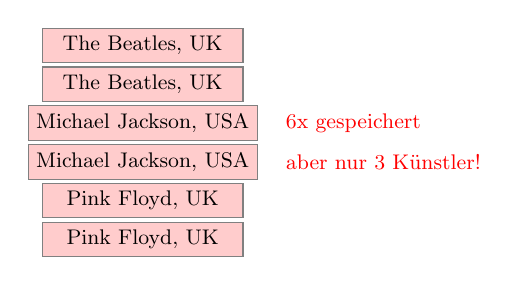
\begin{tikzpicture}[scale=0.85, transform shape]
    % Redundant data visualization using positioning
    \node[tablecell, redundant, minimum width=3cm] (r1) at (0,0) {The Beatles, UK};
    \node[tablecell, redundant, minimum width=3cm, below=0.05cm of r1] (r2) {The Beatles, UK};
    \node[tablecell, redundant, minimum width=3cm, below=0.05cm of r2] (r3) {Michael Jackson, USA};
    \node[tablecell, redundant, minimum width=3cm, below=0.05cm of r3] (r4) {Michael Jackson, USA};
    \node[tablecell, redundant, minimum width=3cm, below=0.05cm of r4] (r5) {Pink Floyd, UK};
    \node[tablecell, redundant, minimum width=3cm, below=0.05cm of r5] (r6) {Pink Floyd, UK};

    \node[font=\small, red, right=0.3cm of r3] {6x gespeichert};
    \node[font=\small, red, right=0.3cm of r4] {aber nur 3 K\"unstler!};
\end{tikzpicture}
\end{column}
\end{columns}

\end{frame}

\begin{frame}{Die Kosten von Redundanz}

\begin{columns}
\begin{column}{0.55\textwidth}
\textbf{Speicherkosten:}
\begin{itemize}
    \item Bei 1000 Alben von 200 Künstlern:
    \item Jeder Künstlername $\sim$ 30 Bytes
    \item Redundant: $1000 \times 30 = 30.000$ Bytes
    \item Optimal: $200 \times 30 = 6.000$ Bytes
    \item \textbf{5x mehr Speicher!}
\end{itemize}

\vspace{0.3cm}

\textbf{Wartungskosten:}
\begin{itemize}
    \item Jede Änderung an vielen Stellen
    \item Zeitaufwand multipliziert sich
    \item Fehlerwahrscheinlichkeit steigt
\end{itemize}
\end{column}

\begin{column}{0.45\textwidth}
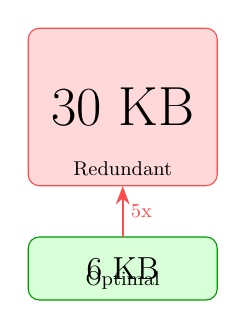
\begin{tikzpicture}[scale=0.8, transform shape]
    % Storage visualization with relative positioning
    \node[goodbox, minimum width=3cm, minimum height=1cm] (good) at (0,0) {};
    \node[above=0.05cm of good.south, font=\small] {Optimal};
    \node at (good.center) {\Large 6 KB};

    \node[alertbox, minimum width=3cm, minimum height=2.5cm, above=0.8cm of good] (bad) {};
    \node[above=0.05cm of bad.south, font=\small] {Redundant};
    \node at (bad.center) {\Huge 30 KB};

    \draw[-{Stealth}, thick, red!70] (good.north) -- node[right, font=\small] {5x} (bad.south);
\end{tikzpicture}
\end{column}
\end{columns}

\vspace{0.3cm}

\begin{alertblock}{Konsistenzkosten}
Eine vergessene Änderung führt zu widersprüchlichen Daten -- das Schlimmste!
\end{alertblock}

\end{frame}

\begin{frame}{Beispiel: Bibliothek}

\textbf{Eine Bibliothek speichert Ausleihen:}

\footnotesize
\begin{tabular}{llllll}
\toprule
\textbf{AusleihNr} & \textbf{Nutzer} & \textbf{Adresse} & \textbf{Buch} & \textbf{Autor} & \textbf{Datum} \\
\midrule
\rowcolor{red!10}
A001 & Müller & Hauptstr. 1 & Der Prozess & Kafka & 2026-01-10 \\
\rowcolor{red!10}
A002 & Müller & Hauptstr. 1 & Das Schloss & Kafka & 2026-01-12 \\
\rowcolor{red!10}
A003 & Müller & Hauptstr. 1 & 1984 & Orwell & 2026-01-15 \\
A004 & Schmidt & Bachweg 7 & Der Prozess & Kafka & 2026-01-16 \\
A005 & Weber & Ringstr. 3 & 1984 & Orwell & 2026-01-18 \\
\bottomrule
\end{tabular}
\normalsize

\vspace{0.3cm}

\textbf{Redundanzen:}
\begin{itemize}
    \item ``Müller, Hauptstr. 1'' erscheint \textbf{3x}
    \item ``Der Prozess, Kafka'' erscheint \textbf{2x}
    \item ``1984, Orwell'' erscheint \textbf{2x}
\end{itemize}

\end{frame}

\begin{frame}{Beispiel: Schule}

\textbf{Eine Schule speichert Kursbelegungen:}

\footnotesize
\begin{tabular}{lllllll}
\toprule
\textbf{Schüler} & \textbf{Klasse} & \textbf{Lehrer\_Kl} & \textbf{Kurs} & \textbf{Kurslehrer} & \textbf{Raum} & \textbf{Note} \\
\midrule
\rowcolor{red!10}
Anna & 10a & Fr. Berg & Mathe & Hr. Klein & R201 & 2 \\
\rowcolor{red!10}
Ben & 10a & Fr. Berg & Mathe & Hr. Klein & R201 & 3 \\
\rowcolor{red!10}
Clara & 10a & Fr. Berg & Mathe & Hr. Klein & R201 & 1 \\
\rowcolor{yellow!20}
Anna & 10a & Fr. Berg & Deutsch & Fr. Groß & R105 & 2 \\
\rowcolor{yellow!20}
Ben & 10a & Fr. Berg & Deutsch & Fr. Groß & R105 & 2 \\
\bottomrule
\end{tabular}
\normalsize

\vspace{0.3cm}

\textbf{Mehrfach gespeichert:}
\begin{itemize}
    \item Klassenlehrer ``Fr. Berg'' -- bei jedem Schüler der 10a
    \item Kursinfos ``Mathe, Hr. Klein, R201'' -- bei jedem Teilnehmer
\end{itemize}

\end{frame}

\begin{frame}{Beispiel: Krankenhaus}

\textbf{Ein Krankenhaus speichert Behandlungen:}

\footnotesize
\begin{tabular}{llllll}
\toprule
\textbf{Patient} & \textbf{Geb.Datum} & \textbf{Arzt} & \textbf{Abteilung} & \textbf{Behandlung} & \textbf{Datum} \\
\midrule
\rowcolor{red!10}
Huber & 15.03.1980 & Dr. Meier & Chirurgie & OP Knie & 10.01.26 \\
\rowcolor{red!10}
Huber & 15.03.1980 & Dr. Meier & Chirurgie & Kontrolle & 20.01.26 \\
\rowcolor{yellow!20}
Fischer & 22.07.1965 & Dr. Schulz & Innere & Bluttest & 12.01.26 \\
\rowcolor{yellow!20}
Fischer & 22.07.1965 & Dr. Schulz & Innere & MRT & 15.01.26 \\
\rowcolor{yellow!20}
Fischer & 22.07.1965 & Dr. Schulz & Innere & Besprechung & 18.01.26 \\
\bottomrule
\end{tabular}
\normalsize

\vspace{0.3cm}

\textbf{Kritische Redundanzen:}
\begin{itemize}
    \item Patientendaten bei jeder Behandlung wiederholt
    \item Arzt-Abteilungs-Zuordnung mehrfach gespeichert
    \item \textbf{Bei Tippfehler:} Falsches Geburtsdatum kann zu Verwechslungen führen!
\end{itemize}

\end{frame}

\begin{frame}{Ein realistischeres Beispiel: Bestellungen}

\footnotesize
\begin{tabular}{llllll}
\toprule
\textbf{BestellNr} & \textbf{Kunde} & \textbf{Adresse} & \textbf{Artikel} & \textbf{Preis} & \textbf{Datum} \\
\midrule
1001 & Müller & Hauptstr. 1 & Laptop & 999 & 2026-01-15 \\
1001 & Müller & Hauptstr. 1 & Maus & 29 & 2026-01-15 \\
1001 & Müller & Hauptstr. 1 & Tastatur & 79 & 2026-01-15 \\
1002 & Schmidt & Bachweg 7 & Monitor & 349 & 2026-01-16 \\
1003 & Müller & Hauptstr. 1 & Webcam & 89 & 2026-01-20 \\
\bottomrule
\end{tabular}
\normalsize

\vspace{0.5cm}

\textbf{Redundanzen identifizieren:}
\begin{itemize}
    \item ``Müller, Hauptstr. 1'' erscheint \textbf{4x}
    \item ``BestellNr 1001, 2026-01-15'' erscheint \textbf{3x}
\end{itemize}

\pause

\begin{alertblock}{Frage}
Was passiert, wenn Herr Müller umzieht?
\end{alertblock}

\end{frame}

\begin{frame}{Bundesliga-Beispiel: Spieler und Vereine}

\textbf{Stellen Sie sich vor, wir erweitern unsere Spieler-Tabelle:}

\footnotesize
\begin{tabular}{lllllll}
\toprule
\textbf{Spieler} & \textbf{Position} & \textbf{Verein} & \textbf{Vereinsort} & \textbf{Stadion} & \textbf{Tore} \\
\midrule
Müller & Sturm & Bayern München & München & Allianz Arena & 8 \\
Neuer & Tor & Bayern München & München & Allianz Arena & 0 \\
Kimmich & Mittelfeld & Bayern München & München & Allianz Arena & 3 \\
Wirtz & Mittelfeld & Bayer Leverkusen & Leverkusen & BayArena & 11 \\
Tah & Abwehr & Bayer Leverkusen & Leverkusen & BayArena & 0 \\
\bottomrule
\end{tabular}
\normalsize

\vspace{0.3cm}

\textbf{Redundanz:}
\begin{itemize}
    \item Vereinsinformationen werden pro Spieler wiederholt
    \item Bei 30 Bayern-Spielern: 30x ``München, Allianz Arena''
\end{itemize}

\end{frame}

\begin{frame}{Vorhersage: Redundanz erkennen}

\textbf{Welche Daten sind in dieser Tabelle redundant gespeichert?}

\footnotesize
\begin{tabular}{llllll}
\toprule
\textbf{Kurs} & \textbf{Dozent} & \textbf{Raum} & \textbf{Student} & \textbf{Matrikelnr} & \textbf{Note} \\
\midrule
DMA & Flath & S103 & Müller & 12345 & 1.7 \\
DMA & Flath & S103 & Schmidt & 12346 & 2.0 \\
DMA & Flath & S103 & Weber & 12347 & 1.3 \\
BWL & Meier & S201 & Müller & 12345 & 2.3 \\
BWL & Meier & S201 & Weber & 12347 & 1.7 \\
\bottomrule
\end{tabular}
\normalsize

\vspace{0.5cm}

\pause

\textbf{Redundant:}
\begin{itemize}
    \item Kursinformationen (Dozent, Raum) pro Teilnehmer wiederholt
    \item Studenteninformationen bei mehreren Kursen wiederholt
\end{itemize}

\end{frame}

%%%%%%%%%%%%%%%%%%%%%%%%%%%%%%%%%%%%%%%%%%%%%%%%%%%%%%%%%%%%%%%%%%%%%%%%%%%%%%%%%%%%%
\section{Phase 3: Anomalien -- Was schief gehen kann}
%%%%%%%%%%%%%%%%%%%%%%%%%%%%%%%%%%%%%%%%%%%%%%%%%%%%%%%%%%%%%%%%%%%%%%%%%%%%%%%%%%%%%

\showagenda{3}

\begin{frame}[fragile]{Anomalie 1: Änderungsanomalie (Update Anomaly)}

\textbf{Problem:} Bei Änderung muss an \textbf{vielen Stellen} geändert werden.

\vspace{0.3cm}

\footnotesize
\begin{tabular}{llll}
\toprule
\textbf{Spieler} & \textbf{Verein} & \textbf{Vereinsort} & \textbf{Stadion} \\
\midrule
Müller & Bayern München & München & Allianz Arena \\
Neuer & Bayern München & München & Allianz Arena \\
Kimmich & Bayern München & München & Allianz Arena \\
\bottomrule
\end{tabular}
\normalsize

\vspace{0.3cm}

\textbf{Szenario:} Bayern zieht in ein neues Stadion um.

\begin{lstlisting}
UPDATE spieler
SET Stadion = 'FC Bayern Arena'
WHERE Verein = 'Bayern München';
\end{lstlisting}

\begin{alertblock}{Gefahr}
Vergisst man \textbf{eine} Zeile, sind die Daten \textbf{inkonsistent}!
\end{alertblock}

\end{frame}

\begin{frame}{Änderungsanomalie: Schritt für Schritt}

\textbf{Szenario:} Die Bibliothek zieht um -- neue Adresse.

\vspace{0.3cm}

\footnotesize
\begin{tabular}{llll}
\toprule
\textbf{Buch} & \textbf{Bibliothek} & \textbf{Adresse} & \textbf{Telefon} \\
\midrule
Der Prozess & Stadtbibliothek & Marktplatz 1 & 0931-123 \\
1984 & Stadtbibliothek & Marktplatz 1 & 0931-123 \\
Faust & Stadtbibliothek & Marktplatz 1 & 0931-123 \\
Harry Potter & Unibibliothek & Campus 5 & 0931-456 \\
\bottomrule
\end{tabular}
\normalsize

\pause
\vspace{0.3cm}

\textbf{Nach dem ``Update'' (ein Fehler passiert):}

\footnotesize
\begin{tabular}{llll}
\toprule
\textbf{Buch} & \textbf{Bibliothek} & \textbf{Adresse} & \textbf{Telefon} \\
\midrule
\rowcolor{green!20}
Der Prozess & Stadtbibliothek & \textbf{Rathausstr. 10} & 0931-123 \\
\rowcolor{green!20}
1984 & Stadtbibliothek & \textbf{Rathausstr. 10} & 0931-123 \\
\rowcolor{red!20}
Faust & Stadtbibliothek & Marktplatz 1 & 0931-123 \\
Harry Potter & Unibibliothek & Campus 5 & 0931-456 \\
\bottomrule
\end{tabular}
\normalsize

\vspace{0.2cm}

\begin{alertblock}{Inkonsistenz!}
Wo ist die Stadtbibliothek jetzt? Marktplatz 1 oder Rathausstr. 10?
\end{alertblock}

\end{frame}

\begin{frame}{Anomalie 2: Einfügeanomalie (Insert Anomaly)}

\textbf{Problem:} Informationen können nicht gespeichert werden, weil \textbf{andere Daten fehlen}.

\vspace{0.5cm}

\textbf{Szenario:} Ein neuer Verein (RB Leipzig II) steigt auf, hat aber noch keine Spieler verpflichtet.

\vspace{0.3cm}

\begin{columns}
\begin{column}{0.5\textwidth}
\footnotesize
\begin{tabular}{lll}
\toprule
\textbf{Spieler} & \textbf{Verein} & \textbf{Stadion} \\
\midrule
Müller & Bayern & Allianz Arena \\
??? & RB Leipzig II & Bruno-Plache \\
\bottomrule
\end{tabular}
\normalsize
\end{column}

\begin{column}{0.5\textwidth}
\begin{alertblock}{Problem}
Ohne Spieler kann der Verein nicht in die Tabelle!

\vspace{0.2cm}

Oder wir brauchen NULL-Werte / Dummy-Daten.
\end{alertblock}
\end{column}
\end{columns}

\vspace{0.3cm}

\textbf{Real-World:} Sie möchten einen Künstler speichern, der noch kein Album hat.

\end{frame}

\begin{frame}{Einfügeanomalie: Weitere Beispiele}

\textbf{Bibliothek:} Neues Buch anschaffen, das noch niemand ausgeliehen hat.

\footnotesize
\begin{tabular}{lllll}
\toprule
\textbf{AusleihNr} & \textbf{Nutzer} & \textbf{Buch} & \textbf{ISBN} & \textbf{Verlag} \\
\midrule
A001 & Müller & Der Prozess & 978-3-123 & Fischer \\
A002 & Schmidt & 1984 & 978-3-456 & Ullstein \\
\rowcolor{yellow!30}
??? & ??? & Neues Buch & 978-3-789 & Suhrkamp \\
\bottomrule
\end{tabular}
\normalsize

\pause
\vspace{0.5cm}

\textbf{Krankenhaus:} Neuen Arzt einstellen, der noch keinen Patienten hat.

\footnotesize
\begin{tabular}{llll}
\toprule
\textbf{Patient} & \textbf{Arzt} & \textbf{Abteilung} & \textbf{Behandlung} \\
\midrule
Huber & Dr. Meier & Chirurgie & OP Knie \\
Fischer & Dr. Schulz & Innere & Bluttest \\
\rowcolor{yellow!30}
??? & Dr. Neu & Neurologie & ??? \\
\bottomrule
\end{tabular}
\normalsize

\vspace{0.2cm}

\begin{alertblock}{Konsequenz}
Wichtige Informationen können nicht gespeichert werden!
\end{alertblock}

\end{frame}

\begin{frame}[fragile]{Anomalie 3: Löschanomalie (Delete Anomaly)}

\textbf{Problem:} Beim Löschen gehen \textbf{ungewollt andere Informationen} verloren.

\vspace{0.5cm}

\footnotesize
\begin{tabular}{llll}
\toprule
\textbf{Spieler} & \textbf{Verein} & \textbf{Vereinsort} & \textbf{Stadion} \\
\midrule
Wirtz & Bayer Leverkusen & Leverkusen & BayArena \\
Tah & Bayer Leverkusen & Leverkusen & BayArena \\
\bottomrule
\end{tabular}
\normalsize

\vspace{0.3cm}

\textbf{Szenario:} Wirtz und Tah wechseln beide ins Ausland.

\begin{lstlisting}
DELETE FROM spieler
WHERE Spieler IN ('Wirtz', 'Tah');
\end{lstlisting}

\begin{alertblock}{Gefahr}
Plötzlich wissen wir nicht mehr, dass Bayer Leverkusen in der BayArena spielt! $\Rightarrow$ Vereinsinformation komplett verloren
\end{alertblock}

\end{frame}

\begin{frame}{Löschanomalie: Schritt für Schritt}

\textbf{Szenario Bibliothek:} Das einzige Exemplar eines Buches wird zurückgegeben.

\vspace{0.3cm}

\footnotesize
\textbf{Vorher:}
\begin{tabular}{lllll}
\toprule
\textbf{AusleihNr} & \textbf{Nutzer} & \textbf{Buch} & \textbf{Autor} & \textbf{Verlag} \\
\midrule
A001 & Müller & Der Prozess & Kafka & Fischer \\
A002 & Schmidt & 1984 & Orwell & Ullstein \\
\rowcolor{red!20}
A003 & Weber & Das Schloss & Kafka & Fischer \\
\bottomrule
\end{tabular}
\normalsize

\pause
\vspace{0.3cm}

\footnotesize
\textbf{Nachher (A003 gelöscht):}
\begin{tabular}{lllll}
\toprule
\textbf{AusleihNr} & \textbf{Nutzer} & \textbf{Buch} & \textbf{Autor} & \textbf{Verlag} \\
\midrule
A001 & Müller & Der Prozess & Kafka & Fischer \\
A002 & Schmidt & 1984 & Orwell & Ullstein \\
\bottomrule
\end{tabular}
\normalsize

\vspace{0.3cm}

\begin{alertblock}{Informationsverlust!}
Das Buch ``Das Schloss'' existiert nicht mehr im System -- obwohl wir es noch haben!
\end{alertblock}

\end{frame}

\begin{frame}{Die drei Anomalien im Überblick}

\begin{center}
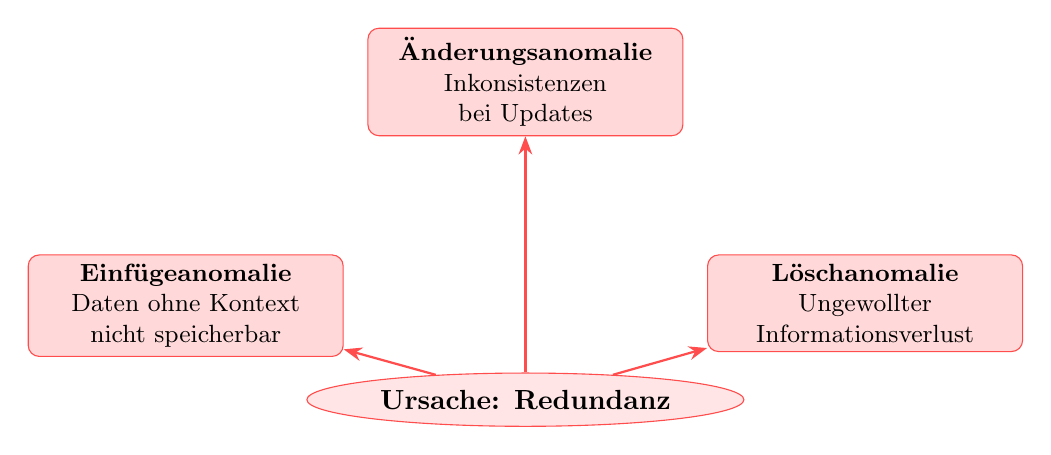
\begin{tikzpicture}[node distance=1.2cm and 0.5cm]
    % Top anomaly centered
    \node[alertbox, minimum width=4cm, minimum height=1.2cm, text width=3.5cm, align=center] (update)
        {\textbf{\"Anderungsanomalie}\\Inkonsistenzen bei Updates};

    % Bottom two anomalies with explicit positioning
    \node[alertbox, minimum width=4cm, minimum height=1.2cm, text width=3.5cm, align=center,
          below left=1.5cm and 0.3cm of update] (insert)
        {\textbf{Einf\"ugeanomalie}\\Daten ohne Kontext\\nicht speicherbar};

    \node[alertbox, minimum width=4cm, minimum height=1.2cm, text width=3.5cm, align=center,
          below right=1.5cm and 0.3cm of update] (delete)
        {\textbf{L\"oschanomalie}\\Ungewollter\\Informationsverlust};

    % Root cause centered below
    \node[draw=red!70, fill=red!10, ellipse, minimum width=3cm,
          below=3cm of update] (root)
        {\textbf{Ursache: Redundanz}};

    % Arrows from root to all three
    \draw[-{Stealth}, thick, red!70] (root) -- (update);
    \draw[-{Stealth}, thick, red!70] (root) -- (insert);
    \draw[-{Stealth}, thick, red!70] (root) -- (delete);
\end{tikzpicture}
\end{center}

\vspace{0.3cm}

\textbf{Merke:} Alle drei Anomalien haben dieselbe Wurzel -- \textbf{Redundanz durch schlechtes Tabellendesign}.

\end{frame}

\begin{frame}{Quiz: Welche Anomalie? (1/2)}

\textbf{Ordnen Sie die Szenarien den Anomalien zu:}

\vspace{0.5cm}

\begin{tabular}{p{8cm}l}
\toprule
\textbf{Szenario} & \textbf{Anomalie?} \\
\midrule
Die Telefonnummer eines Kunden ändert sich, ist aber in 50 Bestellungen gespeichert & ??? \\
\midrule
Ein neuer Lieferant soll erfasst werden, hat aber noch nie geliefert & ??? \\
\midrule
Der letzte Mitarbeiter einer Abteilung kündigt, und wir vergessen den Abteilungsnamen & ??? \\
\bottomrule
\end{tabular}

\vspace{0.5cm}

\pause

\textbf{Lösungen:} Änderungsanomalie, Einfügeanomalie, Löschanomalie

\end{frame}

\begin{frame}{Quiz: Welche Anomalie? (2/2)}

\textbf{Weitere Szenarien -- welche Anomalie liegt vor?}

\vspace{0.3cm}

\begin{enumerate}
    \item Ein Professor geht in Rente. Damit verschwinden alle seine Kurse aus dem System.

    \pause
    \textcolor{red}{$\Rightarrow$ \textbf{Löschanomalie}}

    \vspace{0.2cm}

    \item Die Postleitzahl einer Stadt ändert sich. Sie müssen 500 Kundendatensätze durchsuchen.

    \pause
    \textcolor{red}{$\Rightarrow$ \textbf{Änderungsanomalie}}

    \vspace{0.2cm}

    \item Sie möchten ein neues Produkt ins Sortiment aufnehmen, aber es wurde noch nie bestellt.

    \pause
    \textcolor{red}{$\Rightarrow$ \textbf{Einfügeanomalie}}

    \vspace{0.2cm}

    \item Ein Hotelzimmer wird renoviert. Die neue Zimmerkategorie muss in 200 Buchungsdatensätzen geändert werden.

    \pause
    \textcolor{red}{$\Rightarrow$ \textbf{Änderungsanomalie}}
\end{enumerate}

\end{frame}

\begin{frame}{Vergleich: Schlecht vs. Gut designte Tabelle}

\begin{columns}
\begin{column}{0.5\textwidth}
\textbf{\textcolor{red}{Schlechtes Design:}}

\footnotesize
\begin{tabular}{|l|l|l|}
\hline
\rowcolor{red!20}
\textbf{Kurs} & \textbf{Dozent} & \textbf{Student} \\
\hline
DMA & Flath & Müller \\
\hline
DMA & Flath & Schmidt \\
\hline
DMA & Flath & Weber \\
\hline
BWL & Meier & Müller \\
\hline
\end{tabular}
\normalsize

\vspace{0.2cm}

\textcolor{red}{$\times$} Dozent 3x wiederholt\\
\textcolor{red}{$\times$} Müller 2x wiederholt\\
\textcolor{red}{$\times$} Alle Anomalien möglich
\end{column}

\begin{column}{0.5\textwidth}
\textbf{\textcolor{green!60!black}{Gutes Design:}}

\footnotesize
\begin{tabular}{|l|l|}
\hline
\rowcolor{green!20}
\textbf{Kurs} & \textbf{Dozent} \\
\hline
DMA & Flath \\
\hline
BWL & Meier \\
\hline
\end{tabular}

\vspace{0.1cm}

\begin{tabular}{|l|l|}
\hline
\rowcolor{green!20}
\textbf{Kurs} & \textbf{Student} \\
\hline
DMA & Müller \\
\hline
DMA & Schmidt \\
\hline
DMA & Weber \\
\hline
BWL & Müller \\
\hline
\end{tabular}
\normalsize

\vspace{0.2cm}

\textcolor{green!60!black}{$\checkmark$} Keine Redundanz\\
\textcolor{green!60!black}{$\checkmark$} Keine Anomalien
\end{column}
\end{columns}

\end{frame}

%%%%%%%%%%%%%%%%%%%%%%%%%%%%%%%%%%%%%%%%%%%%%%%%%%%%%%%%%%%%%%%%%%%%%%%%%%%%%%%%%%%%%
\section{Phase 4: Anomalien selbst erleben}
%%%%%%%%%%%%%%%%%%%%%%%%%%%%%%%%%%%%%%%%%%%%%%%%%%%%%%%%%%%%%%%%%%%%%%%%%%%%%%%%%%%%%

\showagenda{4}

{
\setbeamercolor{background canvas}{bg=IMSOrange!15}
\begin{frame}[plain]
\vfill
\begin{center}
{\Huge\color{IMSOrange} Hands-on}\\[1em]
{\Large Anomalien selbst erleben}\\[2em]
{\large\ttfamily marimo: 05-redundanz-probleme.py}\\[1em]
{\normalsize Aufgaben 5.1 -- 5.3}
\end{center}
\vfill
\end{frame}
}

\begin{frame}{Hands-on Aufgaben (Teil 1)}

\textbf{Im Notebook werden Sie:}

\begin{enumerate}
    \item \textbf{Redundanzen identifizieren}
    \begin{itemize}
        \item Eine ``schlechte'' Tabelle analysieren
        \item Doppelte Informationen zählen
    \end{itemize}

    \item \textbf{Änderungsanomalie provozieren}
    \begin{itemize}
        \item Ein UPDATE durchführen
        \item Inkonsistenz erzeugen
    \end{itemize}

    \item \textbf{Löschanomalie erleben}
    \begin{itemize}
        \item Daten löschen
        \item Informationsverlust beobachten
    \end{itemize}
\end{enumerate}

\vspace{0.3cm}

\begin{exampleblock}{Ziel}
Die Probleme am eigenen Leib erfahren -- nicht nur theoretisch verstehen!
\end{exampleblock}

\end{frame}

\begin{frame}{Pause}

\begin{center}
\Large
\textbf{15 Minuten Pause}

\vspace{1cm}

\normalsize
Nach der Pause:\\
Die Lösung -- Daten intelligent aufteilen
\end{center}

\end{frame}

%%%%%%%%%%%%%%%%%%%%%%%%%%%%%%%%%%%%%%%%%%%%%%%%%%%%%%%%%%%%%%%%%%%%%%%%%%%%%%%%%%%%%
\section{Phase 5: Die Lösung -- Daten aufteilen}
%%%%%%%%%%%%%%%%%%%%%%%%%%%%%%%%%%%%%%%%%%%%%%%%%%%%%%%%%%%%%%%%%%%%%%%%%%%%%%%%%%%%%

\showagenda{5}

\begin{frame}{Die Grundidee: Trennung der Konzepte}

\textbf{Problem:} Alles in einer Tabelle $\Rightarrow$ Redundanz

\textbf{Lösung:} \textbf{Jedes ``Ding'' bekommt seine eigene Tabelle!}

\vspace{0.5cm}

\begin{columns}
\begin{column}{0.45\textwidth}
\textbf{Vorher: Eine Tabelle}
\footnotesize
\begin{tabular}{lll}
\toprule
Spieler & Verein & Stadion \\
\midrule
Müller & Bayern & Allianz \\
Neuer & Bayern & Allianz \\
Wirtz & Leverkusen & BayArena \\
\bottomrule
\end{tabular}
\normalsize
\end{column}

\begin{column}{0.55\textwidth}
\textbf{Nachher: Zwei Tabellen}
\footnotesize
\begin{tabular}{ll}
\toprule
\textbf{Spieler} & \textbf{Verein\_ID} \\
\midrule
Müller & 1 \\
Neuer & 1 \\
Wirtz & 2 \\
\bottomrule
\end{tabular}

\vspace{0.2cm}

\begin{tabular}{lll}
\toprule
\textbf{ID} & \textbf{Verein} & \textbf{Stadion} \\
\midrule
1 & Bayern & Allianz \\
2 & Leverkusen & BayArena \\
\bottomrule
\end{tabular}
\normalsize
\end{column}
\end{columns}

\vspace{0.3cm}

$\Rightarrow$ Vereinsinformation nur \textbf{einmal} gespeichert!

\end{frame}

\begin{frame}{Vorteile der Aufteilung}

\begin{columns}
\begin{column}{0.5\textwidth}
\textbf{Änderungen:}
\begin{itemize}
    \item Stadion ändern? $\Rightarrow$ Eine Zeile!
    \item Keine Inkonsistenzen möglich
\end{itemize}

\vspace{0.5cm}

\textbf{Einfügen:}
\begin{itemize}
    \item Neuer Verein ohne Spieler? $\Rightarrow$ Kein Problem!
    \item Informationen unabhängig speicherbar
\end{itemize}

\vspace{0.5cm}

\textbf{Löschen:}
\begin{itemize}
    \item Letzter Spieler weg? $\Rightarrow$ Verein bleibt erhalten!
    \item Kein Informationsverlust
\end{itemize}
\end{column}

\begin{column}{0.5\textwidth}
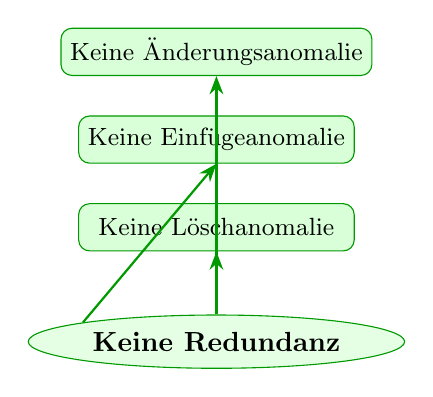
\begin{tikzpicture}[node distance=0.5cm]
    % Use relative positioning for consistent spacing
    \node[goodbox, minimum width=3.5cm] (update) {Keine \"Anderungsanomalie};
    \node[goodbox, minimum width=3.5cm, below=of update] (insert) {Keine Einf\"ugeanomalie};
    \node[goodbox, minimum width=3.5cm, below=of insert] (delete) {Keine L\"oschanomalie};

    \node[draw=green!60!black, fill=green!10, ellipse, minimum width=2.5cm, below=0.8cm of delete] (root)
        {\textbf{Keine Redundanz}};

    \draw[-{Stealth}, thick, green!60!black] (root) -- (delete);
    \draw[-{Stealth}, thick, green!60!black] (root.north west) -- (insert.south);
    \draw[-{Stealth}, thick, green!60!black] (root.north) ++(0,0.1) -- ++(0,0.3) -| (update.south);
\end{tikzpicture}
\end{column}
\end{columns}

\end{frame}

\begin{frame}{Beispiel Bibliothek: Vorher vs. Nachher}

\begin{columns}
\begin{column}{0.5\textwidth}
\textbf{\textcolor{red}{Vorher (eine Tabelle):}}

\footnotesize
\begin{tabular}{|l|l|l|}
\hline
\rowcolor{red!15}
Nutzer & Buch & Autor \\
\hline
Müller & Prozess & Kafka \\
\hline
Müller & Schloss & Kafka \\
\hline
Schmidt & Prozess & Kafka \\
\hline
\end{tabular}
\normalsize

\vspace{0.3cm}
``Kafka'' 3x gespeichert
\end{column}

\begin{column}{0.5\textwidth}
\textbf{\textcolor{green!60!black}{Nachher (drei Tabellen):}}

\footnotesize
\begin{tabular}{|l|l|}
\hline
\rowcolor{green!15}
B\_ID & Titel \\
\hline
1 & Prozess \\
\hline
2 & Schloss \\
\hline
\end{tabular}

\begin{tabular}{|l|l|}
\hline
\rowcolor{green!15}
A\_ID & Name \\
\hline
1 & Kafka \\
\hline
\end{tabular}

\begin{tabular}{|l|l|l|}
\hline
\rowcolor{green!15}
Nutzer & B\_ID & A\_ID \\
\hline
Müller & 1 & 1 \\
\hline
Müller & 2 & 1 \\
\hline
Schmidt & 1 & 1 \\
\hline
\end{tabular}
\normalsize
\end{column}
\end{columns}

\vspace{0.3cm}

\begin{exampleblock}{Ergebnis}
``Kafka'' nur \textbf{einmal} gespeichert -- verknüpft über ID!
\end{exampleblock}

\end{frame}

\begin{frame}{Das Musiksammlung-Beispiel: Verbessert}

\begin{columns}
\begin{column}{0.5\textwidth}
\textbf{Tabelle: Künstler}
\footnotesize
\begin{tabular}{lll}
\toprule
\textbf{ID} & \textbf{Name} & \textbf{Land} \\
\midrule
1 & The Beatles & UK \\
2 & Michael Jackson & USA \\
3 & Pink Floyd & UK \\
\bottomrule
\end{tabular}
\normalsize

\vspace{0.5cm}

\textbf{Tabelle: Alben}
\footnotesize
\begin{tabular}{llll}
\toprule
\textbf{ID} & \textbf{Titel} & \textbf{Jahr} & \textbf{K\_ID} \\
\midrule
1 & Abbey Road & 1969 & 1 \\
2 & Let It Be & 1970 & 1 \\
3 & Thriller & 1982 & 2 \\
4 & Bad & 1987 & 2 \\
5 & Dark Side... & 1973 & 3 \\
\bottomrule
\end{tabular}
\normalsize
\end{column}

\begin{column}{0.5\textwidth}
\textbf{Vorteile:}

\begin{itemize}
    \item ``The Beatles, UK'' nur \textbf{einmal}
    \item Künstler ohne Album möglich
    \item Land ändern = eine Zeile
\end{itemize}

\vspace{0.5cm}

\begin{exampleblock}{Schlüsselprinzip}
Die Spalte \texttt{K\_ID} in Alben \textbf{verweist} auf die Künstler-Tabelle.

\vspace{0.2cm}

$\Rightarrow$ \textbf{Fremdschlüssel}
\end{exampleblock}
\end{column}
\end{columns}

\end{frame}

\begin{frame}{Was ist ein Primärschlüssel?}

\begin{columns}
\begin{column}{0.55\textwidth}
\textbf{Definition:}

Ein \textbf{Primärschlüssel} (Primary Key, PK) ist ein Attribut (oder eine Attributkombination), das jede Zeile einer Tabelle \textbf{eindeutig identifiziert}.

\vspace{0.5cm}

\textbf{Eigenschaften:}
\begin{itemize}
    \item \textbf{Eindeutig:} Keine zwei Zeilen haben denselben Wert
    \item \textbf{Nicht NULL:} Muss immer einen Wert haben
    \item \textbf{Stabil:} Sollte sich nicht ändern
\end{itemize}
\end{column}

\begin{column}{0.45\textwidth}
\footnotesize
\begin{tabular}{|>{\columncolor{IMSBlue!20}}l|l|l|}
\hline
\textbf{ID} & \textbf{Name} & \textbf{Land} \\
\hline
1 & Beatles & UK \\
\hline
2 & Jackson & USA \\
\hline
3 & Pink Floyd & UK \\
\hline
\end{tabular}
\normalsize

\vspace{0.3cm}

\begin{tikzpicture}
    \node[sqlbox, minimum width=2cm] at (0,0) {ID = 1};
    \draw[-{Stealth}, thick, IMSOrange] (1.5,0) -- (2.5,0);
    \node[right] at (2.5,0) {\small genau eine Zeile};
\end{tikzpicture}

\vspace{0.3cm}

\textbf{Beispiele für PKs:}
\begin{itemize}
    \item Matrikelnummer
    \item ISBN
    \item Ausweisnummer
\end{itemize}
\end{column}
\end{columns}

\end{frame}

\begin{frame}{Was ist ein Fremdschlüssel?}

\begin{columns}
\begin{column}{0.55\textwidth}
\textbf{Definition:}

Ein \textbf{Fremdschlüssel} (Foreign Key, FK) ist ein Attribut, das auf den Primärschlüssel einer \textbf{anderen} Tabelle verweist.

\vspace{0.5cm}

\textbf{Zweck:}
\begin{itemize}
    \item Stellt \textbf{Beziehungen} zwischen Tabellen her
    \item Vermeidet Redundanz
    \item Gewährleistet \textbf{referenzielle Integrität}
\end{itemize}

\vspace{0.3cm}

\textbf{Regel:}
Ein FK-Wert muss als PK in der referenzierten Tabelle existieren!
\end{column}

\begin{column}{0.45\textwidth}
\begin{tikzpicture}[node distance=0pt]
    % K\"unstler table - use node distance=0pt for table cells
    \node[draw, fill=IMSBlue!15, minimum width=2.5cm, minimum height=0.6cm] (kt) {\textbf{K\"unstler}};
    \node[draw, fill=IMSBlue!30, minimum width=2.5cm, minimum height=0.5cm, below=of kt] (kid) {\footnotesize ID (PK)};
    \node[draw, minimum width=2.5cm, minimum height=0.5cm, below=of kid] (kn) {\footnotesize Name};

    % Alben table - positioned below with gap
    \node[draw, fill=IMSBlue!15, minimum width=2.5cm, minimum height=0.6cm, below=1cm of kn] (at) {\textbf{Alben}};
    \node[draw, minimum width=2.5cm, minimum height=0.5cm, below=of at] (aid) {\footnotesize ID (PK)};
    \node[draw, minimum width=2.5cm, minimum height=0.5cm, below=of aid] (an) {\footnotesize Titel};
    \node[draw, fill=IMSOrange!30, minimum width=2.5cm, minimum height=0.5cm, below=of an] (afk) {\footnotesize K\_ID (FK)};

    % Arrow - cleaner path from FK to PK
    \draw[-{Stealth}, thick, IMSOrange] (afk.east) -- ++(0.6,0) |- (kid.east);
\end{tikzpicture}
\end{column}
\end{columns}

\end{frame}

\begin{frame}{Schlüssel: Die Verbindung zwischen Tabellen}

\begin{center}
\begin{tikzpicture}[node distance=0.15cm]
    % K\"unstler table - left side
    \node[entitybox, minimum width=4cm] (k) {\textbf{K\"unstler}};
    \node[below=0.2cm of k, font=\small\ttfamily] (kid) {ID (PK)};
    \node[below=of kid, font=\small\ttfamily] (kname) {Name};
    \node[below=of kname, font=\small\ttfamily] (kland) {Land};

    % Alben table - right side with horizontal offset
    \node[entitybox, minimum width=4cm, right=4cm of k] (a) {\textbf{Alben}};
    \node[below=0.2cm of a, font=\small\ttfamily] (aid) {ID (PK)};
    \node[below=of aid, font=\small\ttfamily] (atitel) {Titel};
    \node[below=of atitel, font=\small\ttfamily] (fk) {K\"unstler\_ID (FK)};

    % Arrow - from FK to PK with proper routing
    \draw[-{Stealth}, thick, IMSOrange] (fk.west) -- ++(-0.8,0) |- (kid.east);
\end{tikzpicture}
\end{center}

\vspace{0.3cm}

\begin{columns}
\begin{column}{0.5\textwidth}
\textbf{Primärschlüssel (PK):}
\begin{itemize}
    \item Identifiziert jede Zeile \textbf{eindeutig}
    \item Keine Duplikate erlaubt
    \item Darf nicht NULL sein
\end{itemize}
\end{column}

\begin{column}{0.5\textwidth}
\textbf{Fremdschlüssel (FK):}
\begin{itemize}
    \item Verweist auf PK einer anderen Tabelle
    \item Stellt \textbf{Beziehung} her
    \item Kann sich wiederholen
\end{itemize}
\end{column}
\end{columns}

\end{frame}

\begin{frame}[fragile]{SQL: Tabellen mit Schlüsseln erstellen}

\begin{lstlisting}
CREATE TABLE kuenstler (
    id INTEGER PRIMARY KEY,
    name TEXT NOT NULL,
    land TEXT
);

CREATE TABLE alben (
    id INTEGER PRIMARY KEY,
    titel TEXT NOT NULL,
    jahr INTEGER,
    kuenstler_id INTEGER,
    FOREIGN KEY (kuenstler_id) REFERENCES kuenstler(id)
);
\end{lstlisting}

\vspace{0.3cm}

\textbf{Wichtige Konzepte:}
\begin{itemize}
    \item \texttt{PRIMARY KEY}: Eindeutige Identifikation
    \item \texttt{FOREIGN KEY}: Referenz auf andere Tabelle
    \item \texttt{REFERENCES}: Gibt an, auf welche Tabelle/Spalte verwiesen wird
\end{itemize}

\end{frame}

\begin{frame}{Referenzielle Integrität}

\textbf{Definition:} Jeder Fremdschlüsselwert muss auf einen existierenden Primärschlüssel verweisen.

\vspace{0.5cm}

\begin{columns}
\begin{column}{0.5\textwidth}
\textbf{\textcolor{green!60!black}{Gültig:}}

\footnotesize
\begin{tabular}{|l|l|}
\hline
\rowcolor{green!20}
ID & Name \\
\hline
1 & Beatles \\
\hline
2 & Jackson \\
\hline
\end{tabular}

\begin{tabular}{|l|l|}
\hline
\rowcolor{green!20}
Titel & K\_ID \\
\hline
Abbey Road & 1 \\
\hline
Thriller & 2 \\
\hline
\end{tabular}
\normalsize

\vspace{0.2cm}
\textcolor{green!60!black}{$\checkmark$} K\_ID 1 und 2 existieren
\end{column}

\begin{column}{0.5\textwidth}
\textbf{\textcolor{red}{Ungültig:}}

\footnotesize
\begin{tabular}{|l|l|}
\hline
ID & Name \\
\hline
1 & Beatles \\
\hline
2 & Jackson \\
\hline
\end{tabular}

\begin{tabular}{|l|l|}
\hline
Titel & K\_ID \\
\hline
Abbey Road & 1 \\
\hline
\rowcolor{red!20}
Neues Album & \textbf{99} \\
\hline
\end{tabular}
\normalsize

\vspace{0.2cm}
\textcolor{red}{$\times$} K\_ID 99 existiert nicht!
\end{column}
\end{columns}

\vspace{0.3cm}

\begin{alertblock}{Schutz durch das DBMS}
Die Datenbank \textbf{verhindert} ungültige Fremdschlüsselwerte automatisch!
\end{alertblock}

\end{frame}

%%%%%%%%%%%%%%%%%%%%%%%%%%%%%%%%%%%%%%%%%%%%%%%%%%%%%%%%%%%%%%%%%%%%%%%%%%%%%%%%%%%%%
\section{Phase 6: Erste Schritte zur Modellierung}
%%%%%%%%%%%%%%%%%%%%%%%%%%%%%%%%%%%%%%%%%%%%%%%%%%%%%%%%%%%%%%%%%%%%%%%%%%%%%%%%%%%%%

\showagenda{6}

\begin{frame}{Entitäten und Beziehungen}

\textbf{Kernfrage der Datenmodellierung:}

\begin{enumerate}
    \item Welche ``Dinge'' (Entitäten) gibt es?
    \item Wie hängen sie zusammen (Beziehungen)?
\end{enumerate}

\vspace{0.5cm}

\begin{center}
\begin{tikzpicture}[node distance=3cm]
    \node[entitybox] (k) {Künstler};
    \node[relationbox, right=of k] (rel) {hat};
    \node[entitybox, right=of rel] (a) {Album};

    \draw[thick] (k) -- (rel);
    \draw[thick] (rel) -- (a);

    \node[below=0.3cm of k, font=\small, gray] {Entität};
    \node[below=0.3cm of rel, font=\small, gray] {Beziehung};
    \node[below=0.3cm of a, font=\small, gray] {Entität};
\end{tikzpicture}
\end{center}

\vspace{0.3cm}

\textbf{Entität:} Ein ``Ding'' der realen Welt (Künstler, Album, Spieler, Verein)

\textbf{Beziehung:} Verbindung zwischen Entitäten (hat, gehört\_zu, spielt\_für)

\end{frame}

\begin{frame}{Kardinalitäten: Wie viele?}

\textbf{Wichtige Frage:} Wie viele Entitäten stehen in Beziehung?

\vspace{0.5cm}

\begin{center}
\begin{tikzpicture}[node distance=2.5cm]
    % 1:N
    \node[entitybox, minimum width=2.5cm] (k) {Künstler};
    \node[relationbox, right=of k] (rel) {hat};
    \node[entitybox, minimum width=2cm, right=of rel] (a) {Album};

    \draw[thick] (k) -- node[above, font=\small] {1} (rel);
    \draw[thick] (rel) -- node[above, font=\small] {N} (a);

    \node[below=0.5cm of rel, font=\small] {``Ein Künstler hat \textbf{mehrere} Alben''};
    \node[below=1cm of rel, font=\small] {``Ein Album gehört zu \textbf{einem} Künstler''};
\end{tikzpicture}
\end{center}

\vspace{0.5cm}

\textbf{Typische Kardinalitäten:}
\begin{itemize}
    \item \textbf{1:1} -- Ein Bürger hat einen Personalausweis
    \item \textbf{1:N} -- Ein Verein hat mehrere Spieler
    \item \textbf{M:N} -- Studenten besuchen Kurse (mehrere zu mehreren)
\end{itemize}

\end{frame}

\begin{frame}{Beispiel: Bundesliga-Datenmodell}

\begin{center}
\begin{tikzpicture}[node distance=1.5cm and 2cm, scale=0.9, transform shape]
    % Entities - clearer 2x2 grid layout
    \node[entitybox] (v) {Verein};
    \node[entitybox, right=4.5cm of v] (s) {Spieler};
    \node[entitybox, below=2.5cm of v] (st) {Stadion};
    \node[entitybox, below=2.5cm of s] (sp) {Spiel};

    % Relationships - centered between entities
    \node[relationbox] (hat) at ($(v)!0.5!(s)$) {hat};
    \node[relationbox] (spielt) at ($(v)!0.5!(st)$) {spielt in};

    % Lines for hat and spielt relationships
    \draw[thick] (v) -- node[above, font=\small] {1} (hat);
    \draw[thick] (hat) -- node[above, font=\small] {N} (s);
    \draw[thick] (v) -- node[left, font=\small] {N} (spielt);
    \draw[thick] (spielt) -- node[left, font=\small] {1} (st);

    % Spiel relationship - simplified with cleaner path
    \node[relationbox, below=0.6cm of sp] (nimmt) {nimmt teil};
    \draw[thick] (v.south) -- ++(0,-0.4) -| node[pos=0.25, above, font=\small] {2} (nimmt.west);
    \draw[thick] (nimmt) -- node[right, font=\small] {1} (sp);
\end{tikzpicture}
\end{center}

\vspace{0.3cm}

\textbf{Entitäten:} Verein, Spieler, Stadion, Spiel

\textbf{Beziehungen:} hat (1:N), spielt\_in (N:1), nimmt\_teil (2:1)

\end{frame}

\begin{frame}{Vorhersage: Kardinalität bestimmen}

\textbf{Welche Kardinalität haben diese Beziehungen?}

\vspace{0.5cm}

\begin{tabular}{p{7cm}l}
\toprule
\textbf{Beziehung} & \textbf{Kardinalität} \\
\midrule
Ein Buch hat einen Verlag & ??? \\
Ein Student belegt Kurse & ??? \\
Eine Person hat eine Sozialversicherungsnummer & ??? \\
Ein Dozent hält Vorlesungen & ??? \\
\bottomrule
\end{tabular}

\vspace{0.5cm}

\pause

\textbf{Lösungen:}
\begin{itemize}
    \item Buch -- Verlag: N:1 (viele Bücher, ein Verlag)
    \item Student -- Kurse: M:N (viele zu vielen)
    \item Person -- SVN: 1:1 (eindeutig)
    \item Dozent -- Vorlesungen: 1:N (ein Dozent, viele Vorlesungen)
\end{itemize}

\end{frame}

{
\setbeamercolor{background canvas}{bg=IMSOrange!15}
\begin{frame}[plain]
\vfill
\begin{center}
{\Huge\color{IMSOrange} Hands-on}\\[1em]
{\Large Tabellen aufteilen}\\[2em]
{\large\ttfamily marimo: 05-redundanz-probleme.py}\\[1em]
{\normalsize Aufgaben 5.4 -- 5.6}
\end{center}
\vfill
\end{frame}
}

\begin{frame}{Hands-on: Verbessertes Design}

\textbf{Im zweiten Teil des Notebooks:}

\begin{enumerate}
    \item \textbf{Tabellen aufteilen}
    \begin{itemize}
        \item Die ``schlechte'' Tabelle in zwei Tabellen zerlegen
        \item Fremdschlüssel einführen
    \end{itemize}

    \item \textbf{Änderung testen}
    \begin{itemize}
        \item Dieselbe Änderung wie vorher durchführen
        \item Sehen: Nur eine Zeile betroffen!
    \end{itemize}

    \item \textbf{Daten abfragen}
    \begin{itemize}
        \item Vorschau auf JOINs (nächste Vorlesung)
        \item Wie kombiniert man die Tabellen wieder?
    \end{itemize}
\end{enumerate}

\end{frame}

%%%%%%%%%%%%%%%%%%%%%%%%%%%%%%%%%%%%%%%%%%%%%%%%%%%%%%%%%%%%%%%%%%%%%%%%%%%%%%%%%%%%%
\section{Phase 7: Zusammenfassung \& Ausblick}
%%%%%%%%%%%%%%%%%%%%%%%%%%%%%%%%%%%%%%%%%%%%%%%%%%%%%%%%%%%%%%%%%%%%%%%%%%%%%%%%%%%%%

\showagenda{7}

\begin{frame}{Zusammenfassung: Was wir gelernt haben}

\begin{columns}
\begin{column}{0.5\textwidth}
\textbf{Probleme der Mega-Tabelle:}
\begin{itemize}
    \item Redundanz (gleiche Daten mehrfach)
    \item Änderungsanomalie
    \item Einfügeanomalie
    \item Löschanomalie
\end{itemize}

\vspace{0.3cm}

\textbf{Lösung:}
\begin{itemize}
    \item Daten in mehrere Tabellen aufteilen
    \item Jede Entität eigene Tabelle
    \item Verbindung durch Schlüssel
\end{itemize}
\end{column}

\begin{column}{0.5\textwidth}
\textbf{Neue Konzepte:}
\begin{itemize}
    \item \textbf{Entität}: ``Ding'' der realen Welt
    \item \textbf{Beziehung}: Verbindung zwischen Entitäten
    \item \textbf{Primärschlüssel}: Eindeutige ID
    \item \textbf{Fremdschlüssel}: Verweis auf andere Tabelle
    \item \textbf{Kardinalität}: 1:1, 1:N, M:N
\end{itemize}
\end{column}
\end{columns}

\end{frame}

\begin{frame}{Die wichtigsten Begriffe}

\begin{center}
\begin{tabular}{ll}
\toprule
\textbf{Begriff} & \textbf{Bedeutung} \\
\midrule
Redundanz & Mehrfache Speicherung derselben Information \\
Änderungsanomalie & Inkonsistenzen bei Updates \\
Einfügeanomalie & Daten ohne Kontext nicht speicherbar \\
Löschanomalie & Ungewollter Informationsverlust beim Löschen \\
\midrule
Entität & ``Ding'' der realen Welt (wird zu Tabelle) \\
Primärschlüssel (PK) & Eindeutige Identifikation einer Zeile \\
Fremdschlüssel (FK) & Verweis auf PK einer anderen Tabelle \\
Kardinalität & Anzahl der Beziehungen (1:1, 1:N, M:N) \\
Referenzielle Integrität & FK-Werte müssen als PK existieren \\
\bottomrule
\end{tabular}
\end{center}

\end{frame}

\begin{frame}{Ausblick: Die nächsten Vorlesungen}

\textbf{Vorlesung 6: Entity-Relationship-Modellierung}
\begin{itemize}
    \item Formale ER-Notation (Chen / Krähenfuß)
    \item Komplexe Modelle erstellen
    \item Übung: Eigene Modelle zeichnen
\end{itemize}

\vspace{0.5cm}

\textbf{Vorlesung 7: Relationales Modell}
\begin{itemize}
    \item ER-Modelle in Tabellen umwandeln
    \item CREATE TABLE Statements
    \item Integritätsbedingungen
\end{itemize}

\vspace{0.5cm}

\begin{exampleblock}{Vorschau}
\textbf{Vorlesung 9: JOINs} -- Wie kombiniert man mehrere Tabellen in Abfragen?
\end{exampleblock}

\end{frame}

\begin{frame}{Vorhersage: Abschlussquiz}

\textbf{1. Welche Anomalie tritt auf, wenn man einen Wert ändert und er an mehreren Stellen steht?}
\begin{itemize}
    \item[A)] Einfügeanomalie
    \item[B)] Änderungsanomalie
    \item[C)] Löschanomalie
\end{itemize}

\pause
\textbf{Antwort: B}

\vspace{0.3cm}

\textbf{2. Welcher Schlüsseltyp verweist auf einen Primärschlüssel in einer anderen Tabelle?}
\begin{itemize}
    \item[A)] Superkey
    \item[B)] Primärschlüssel
    \item[C)] Fremdschlüssel
\end{itemize}

\pause
\textbf{Antwort: C}

\end{frame}

\begin{frame}{Vorhersage: Abschlussquiz (Fortsetzung)}

\textbf{3. Was ist die Hauptursache aller drei Anomalien?}
\begin{itemize}
    \item[A)] Zu viele Tabellen
    \item[B)] Redundanz
    \item[C)] Fehlende Primärschlüssel
\end{itemize}

\pause
\textbf{Antwort: B}

\vspace{0.3cm}

\textbf{4. Ein Künstler kann mehrere Alben haben, aber jedes Album gehört zu genau einem Künstler. Welche Kardinalität liegt vor?}
\begin{itemize}
    \item[A)] 1:1
    \item[B)] 1:N
    \item[C)] M:N
\end{itemize}

\pause
\textbf{Antwort: B}

\end{frame}

\begin{frame}

\begin{center}
\Large
\textbf{Fragen?}

\vspace{1cm}

\normalsize
Nächste Woche: Entity-Relationship-Modellierung

\vspace{0.5cm}

\textit{``Gutes Datenbankdesign ist wie gute Architektur --\\
man sieht es erst, wenn etwas schief geht.''}
\end{center}

\end{frame}

\end{document}
